\documentclass{ieeeaccess}
\usepackage{cite}
\usepackage{amsmath,amssymb,amsfonts}
\usepackage{algorithmic}
\usepackage{graphicx}
\usepackage{units}
\usepackage{color}
\usepackage{textcomp}
\usepackage{caption}
\usepackage{etoolbox}
\usepackage{placeins}
\usepackage{tikz}
	\NewSpotColorSpace{PANTONE}
	\AddSpotColor{PANTONE} {PANTONE3015C} {PANTONE\SpotSpace 3015\SpotSpace C} {1 0.3 0 0.2}
	\SetPageColorSpace{PANTONE}%


\begin{document}

\history{Date of current version Monday 20, 2020.}
\doi{PLACEHOLDER}

\title{EEET 4075 Mechatronic System Design 2 - Project Report}
\author{\uppercase{Michael J. Duke}\authorrefmark{1}}
\address[1]{University of South Australia, Mawson Lakes, SA 5095 Australia (e-mail: dukmj002@mymail.unisa.edu.au)}
\tfootnote{This work was supported in part by the University of South Australia}

\markboth
{Michael J. Duke: EEET 4075 Mechatronic System Design 2 - Project Report}
{Michael J. Duke: EEET 4075 Mechatronic System Design 2 - Project Report}

\titlepgskip=-15pt

\maketitle

\section{Introduction}
\label{sec:introduction}
\PARstart{M}{ultirate} Extended Kalman Filters and absolute versus relative (dead reckoning) localisation.

\section{Related Works}
\label{sec:rel}
Several different ways to combine the estimations of different sensors, difficulties with multi-rate systems. Variants or modifications on EKF and UKF, compare and contrast, computational cost, relative accuracy, limitations. maybe compare to particle filters as well? Need for an initial estimate of position and heading. Beacon based navigation.

\section{Methodology}
\label{sec:meth}
\subsection{System Model}
	\begin{equation}
	\label{eq:xsys}
		\boldsymbol{x}_{ k} = 
		\begin{bmatrix}
			x _{ k}	\\
			y_{ k}		\\
			\theta_{ k}
		\end{bmatrix}
		=
		\begin{bmatrix}
			x_{k-1}+Tv\cos{\left(\theta_{k-1}\right)}								\\
			y_{k-1}+Tv\sin{\left(\theta_{k-1}\right)}								\\
			\theta_{k-1} + T\omega
		\end{bmatrix}
	\end{equation}
	
	\begin{equation}
	\label{eq:Fsys}
		\boldsymbol{F}_{k} = \frac{\partial\boldsymbol{f}}{\partial\boldsymbol{x_{k-1}}}
		=
		\begin{bmatrix}
			1	&0	&-Tv\sin{\left(\theta_{k-1}\right)}	\\
			0	&1	&Tv\cos{\left(\theta_{k-1}\right)}	\\
			0	&0	&1
		\end{bmatrix}
	\end{equation}

\subsection{Measurement}

	\begin{equation}
	\label{eq:delts}
		\delta s_{k} = \frac{s_{r,k} - s_{r,k-1} + s_{l,k} - s_{l,k-1}}{2}
	\end{equation}
	
	\begin{equation}
	\label{eq:deltth}
		\delta \theta_{k} = \frac{s_{r,k} - s_{r,k-1} + s_{l,k} - s_{l,k-1}}{b}
	\end{equation}
	where $b$ is the wheelbase in m,
	\begin{equation}
	\label{eq:b}
		b = 0.287
	\end{equation}
	
	\begin{equation}
	\label{eq:hsys}
		\boldsymbol{h}_{ k} =
		\begin{bmatrix}
			\delta s_{k} 		\\
			\delta\theta_{k}	\\
			\omega_{k}
		\end{bmatrix}
		=
		\begin{bmatrix}
			\sqrt{\left(x_{k} - x_{k-1}\right)^{2} + \left(y_{k} - y_{k-1}\right)^{2}}	\\
			\theta_{k} - \theta_{k-1}								\\
			\frac{\theta_{k}-\theta_{k-1}}{T}
		\end{bmatrix}
	\end{equation}
	
	\begin{equation}
	\label{eq:Hsys}
		\boldsymbol{H}_{k}	=
		\begin{bmatrix}
			\frac{x_{k}-x_{k-1}}{\sqrt{\left( x_{k} - x_{k-1} \right)^{2}+\left( y_{k} - y_{k-1} \right)^{2}}}	&0	&0		\\
			\frac{y_{k}-y_{k-1}}{\sqrt{\left( x_{k} - x_{k-1} \right)^{2}+\left( y_{k} - y_{k-1} \right)^{2}}}	&0	&0		\\
			0															&1	&\frac{1}{T}	\\
		\end{bmatrix}^{\top}
	\end{equation}

\subsection{LiDaR}
	To estimate the orientation of the turtlebot, the angle to the closest beacon is used as a correction.
	
	To estimate the position of the turtlebot, the intersection of two circles is calculated knowing their center coordinates and radii.
	\begin{equation}
	\begin{aligned}
		\left(x-x_{1}\right)^{2} + \left(y-y_{1}\right)^{2}=r_{1}^{2}	\\
		\left(x-x_{2}\right)^{2} + \left(y-y_{2}\right)^{2}=r_{2}^{2}
	\end{aligned}
	\end{equation}
	Rearranging, and with the assumption that $x_{1}=x_{2}$  in both cases we get
	\begin{equation}
		y = -\frac{r_{1}^{2}-r_{2}^{2}-y_{1}^{2}+y_{2}^{2}}{2\left(y_{1}-y_{2}\right)}
	\end{equation}
	
	\begin{equation}
	\begin{aligned}
		x 		&= \pm \frac{\sqrt{\beta_{1}\beta_{2}}}{2\left(y_{1}-y_{2}\right)}	\\
		\beta_{1} 	&= \left(r_{1}+r_{2}\right)^{2}-\left(y_{1}-y_{2}\right)^{2}		\\
		\beta_{2} 	&=\left(y_{1}-y_{2}\right)^{2}-\left(r_{1}-r_{2}\right)^{2}
	\end{aligned}
	\end{equation}
	As we know the fence around which the bot cannot escape, one of the possible positions can be eliminated, leaving BLAH if using the left beacons, and BLAH if using the right beacons.
	\begin{equation}
		x 		= \frac{\sqrt{\beta_{1}\beta_{2}}}{2\left(y_{1}-y_{2}\right)}
	\end{equation}
	\begin{equation}
		x 		= 3.5-\frac{\sqrt{\beta_{1}\beta_{2}}}{2\left(y_{1}-y_{2}\right)}
	\end{equation}
	
	
	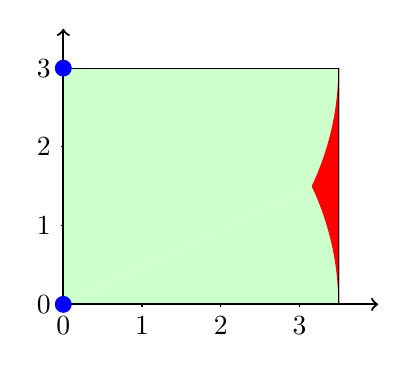
\begin{tikzpicture}
%		\draw[step=1cm,lightgray,very thin] (-0.9,-0.9) grid (4.9, 3.9);
		\foreach \x in {0,1,2,3}
 			\draw (\x cm,1pt) -- (\x cm,-1pt) node[anchor=north] {$\x$};
		\foreach \y in {0,1,2,3}
			\draw (1pt,\y cm) -- (-1pt,\y cm) node[anchor=east] {$\y$};
		\filldraw[fill=green!20!white, green!20!white] (0,3) -- ({3.5*cos(asin(1.5/3.5))},1.5) arc ({360-asin(1.5/3.5)}:360:3.5cm);
		\filldraw[fill=green!20!white, green!20!white] (0,0) -- (3.5,0) arc (0:{asin(1.5/3.5)}:3.5cm);
		\filldraw[fill=green!20!white, green!20!white] (0,0) -- (0,3) -- ({3.5*cos(asin(1.5/3.5))},1.5);
		\filldraw[fill=red, red] ({3.5*cos(asin(1.5/3.5))},1.5) arc ({360-asin(1.5/3.5)}:360:3.5cm) -- (3.5,0) arc (0:{asin(1.5/3.5)}:3.5cm);
		\draw (0,0) -- (3.5,0) -- (3.5,3) -- (0,3) -- (0,0);
		\draw[thick,->] (0,0) -- (4,0);
		\draw[thick,->] (0,0) -- (0,3.5);
		\filldraw[fill=blue, blue] (0,0) circle (0.1cm);
		\filldraw[fill=blue, blue] (0,3) circle (0.1cm);
	\end{tikzpicture}
	
\subsection{EKF}

	a priori estimate
	\begin{equation}
	\label{eq:x-}
		\hat{\boldsymbol{x}}_{k}^{-}=\boldsymbol{f}_{k-1}\left(\hat{\boldsymbol{x}}^{+}_{k-1},\,\boldsymbol{u}_{k-1}\right)
	\end{equation}
	
	\begin{equation}
	\label{eq:P+}
		\boldsymbol{P}_{k}^{-} = \boldsymbol{F}_{k-1}\boldsymbol{P}_{k-1}^{+}\boldsymbol{F}_{k-1}^{\top} + \boldsymbol{Q}_{k-1}
	\end{equation}
	
	Kalman gain update,
	\begin{equation}
	\label{eq:K}
		\boldsymbol{K}_{1,\,k} = \boldsymbol{P}_{k}^{-}\boldsymbol{H}_{1,\,k}^{\top}\left(\boldsymbol{H}_{1,\,k}\boldsymbol{P}{1,\,k}^{-}\boldsymbol{H}_{1,\,k}^{\top} + \boldsymbol{R}_{1,\,k} \right)^{-1}
	\end{equation}
	
	a posteriori estimate,
	\begin{equation}
	\label{eq:x+}
		\hat{\boldsymbol{x}}_{k}^{+}=\hat{\boldsymbol{x}}_{k}^{-} + \boldsymbol{K}_{1,\,k}\left(\boldsymbol{y}_{1,\,k}- \boldsymbol{h}_{1,\,k}\right)
	\end{equation}
	
	\begin{equation}
	\label{eq:p+}
		\boldsymbol{P}_{1,\,k}^{+} = \left(\boldsymbol{I} - \boldsymbol{K}_{1,\,k}\boldsymbol{H}_{1,\,k}\right)\boldsymbol{P}_{1,\,k}^{-}
	\end{equation}
	When the secondary measurement is received, the kalman gain, error, and state estimate are updated
	\begin{equation}
	\label{eq:K2}
		\boldsymbol{K}_{2,\,k} = \boldsymbol{P}_{1,\,k}^{-}\boldsymbol{H}_{2,\,k}^{\top}\left(\boldsymbol{H}_{2,\,k}\boldsymbol{P}_{1,\,k}^{-}\boldsymbol{H}_{2,\,k}^{\top} + \boldsymbol{R}_{2,\,k} \right)^{-1}
	\end{equation}
	\begin{equation}
	\label{eq:p2+}
		\boldsymbol{P}_{2,\,k}^{+} = \left(\boldsymbol{I} - \boldsymbol{K}_{2,\,k}\boldsymbol{H}_{2,\,k}\right)\boldsymbol{P}_{1,\,k}^{-}
	\end{equation}
	\begin{equation}
	\label{eq:x+}
		\hat{\boldsymbol{x}}_{k}^{+}=\hat{\boldsymbol{x}}_{k}^{-} + \boldsymbol{K}_{1,\,k}\left(\boldsymbol{y}_{1,\,k}- \boldsymbol{h}_{1,\,k}\right) + \boldsymbol{K}_{2,\,k}\left(\boldsymbol{y}_{2,\,k}-\boldsymbol{H}_{2,\,k}\hat{\boldsymbol{x}}_{k}^{-}\right)
	\end{equation}
\section{Results and Discussion}
\label{sec:res}


\section{Conclusion}
\label{sec:con}


\section{References}
Trajectory Planning for Nonholonomic Mobile Robot Using Extended Kalman Filter\par
Integrated Indoor Navigation System for Ground Vehicles With Automatic 3-D Alignment and Position Initialization.\par
Incorporating delayed and infrequent measurements in Extended Kalman Filter based nonlinear state estimation.\par

\EOD

\end{document}
